\chapter{Introduction}

\section{Course Structure \& Logistics}
\begin{center}
    \begin{tikzpicture}
        \clip (0,0)  circle (2cm) ;
        \node[anchor=center] at (0,-0.5) {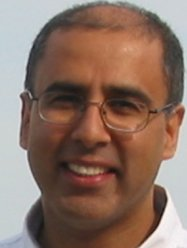
\includegraphics[width=4.5cm]{introduction/images/drdulay.jpg}};
    \end{tikzpicture}
    \centerline{\textbf{Dr Narankar Dulay}}
\end{center}
The module is taught by \href{http://wp.doc.ic.ac.uk/nd/}{Dr Narankar Dulay}.
\\
\\ \textbf{Theory} For weeks 2 $\to$ 10:
\begin{itemize}
    \item Elixir (learning programming language)
    \item Introduction
    \item Reliable Broadcast
    \item FIFO, casual and total order Broadcast
    \item Consensus
    \item Flip Improbability Result
    \item Temporal Logic of Actions
    \item Modelling Broadcast
    \item Modelling Consensus
\end{itemize}

\section{Course Resources}
The \href{https://www.doc.ic.ac.uk/~nd/dal/}{course website} contains all available slides and notes.

\section{Distributed Systems}
\begin{definitionbox}{Distributed System}
    A set of processes connected by a network, communicating by message passing and with no shared physical clock.
    \begin{itemize}
        \item No total order on events by time (no shared clock)
        \item No shared memory.
        \item Network is logical - processes may be on the same OS process, same VM, same machine different machines communicating over a physical network. 
    \end{itemize}
\end{definitionbox}

Distributed systems must contend with the inherit uncertainty (failure, communication delay and an inconsistent view of the system's state) in communication between potentially physically independent processes (fallible machines, networks and software).

\begin{sidenotebox}{Leisle Lamport}
    A computer scientist and mathematician, credited with creating TLA (used on this course), as well as being the initial developer of latex (used for these notes).
    \begin{quote}
        "
            There has been considerable debate over the years 
            about what constitutes a distributed system. It 
            would appear that the following definition has been 
            adopted at SRC:

            A distributed system is one in which the failure of 
            a computer you didn't even know existed can render 
            your own computer unusable.
        "
    \end{quote}
\end{sidenotebox}

\unfinished